
\chapter{Aircraft Physical Models}
\label{chap:phy}

To evaluate the size and performance of both gas and solar-electric powered aircraft, underlying physics models are used.  
Environmental, aircraft performance, and structural models are used in the optimization model to capture the effects of the requirements on the size and design of the aircraft.
Equations from these models are expressed in a GP-compatible form to enable their use in the optimization. 
Understanding the models that are used in a GP is important because the solution to a GP is only as accurate as the models that are used to construct the program.  
To obtain higher fidelity results from the optimization, more detailed models can be implemented. 

\section{Shared Physical Models}

The models described in this section were applied to both the gas powered and solar-electric powered aircraft models. 

\subsection{Steady Level Flight}

Both the gas and solar powered aircraft are assumed to be in steady level flight,\cite{hoburgthesis}

\begin{align}
    \label{e:slfthrust}
    T &\geq \frac{1}{2} \rho V^2 C_D S\\
    \label{e:slfweight}
    W &= \frac{1}{2} \rho V^2 C_L S. 
\end{align}

The shaft power produced by the engine or motor can be expressed as  

\begin{equation}
    \label{e:slfpower}
    P_{\text{shaft}} = \frac{TV}{\eta_{\text{prop}}}
    \end{equation}

    where the propulsive efficiency is assumed to be a constant, $\eta_{\text{prop}} = 0.8$. 

\subsection{Aerodynamics}

The aircraft aerodynamics is modeled as a drag build up of the non-wing drag, wing profile drag, and induced drag coefficients, 

\begin{equation}
    \label{e:aerodragb}
    C_D \geq C_{d_0} + c_{d_p} + \frac{C_L^2}{\pi e A}.
    \end{equation}

where the span efficiency factor is assumed to be constant, $e=0.9$. 
The non-wing drag coefficient $C_{d_0}$, is estimated as a drag build up from the fuselage, tail boom, and horizontal and vertical surfaces discussed later.
    
To estimate the wing profile drag, a posynomial fit is made of the drag polar of the selected \emph{JH01} airfoil, Equation~\ref{e:aerodragprof} (See Appendix \ref{app:jho} for a discussion of the airfoil choice). 
Drag polars were produced using XFOIL\cite{xfoil} at various Reynolds and the data was then fit to a posynomial equation. (See Appendix \ref{app:fits})
    The XFOIL drag polar data is compared to the posynomial fit in Figure~\ref{f:JH01polar}.

    \begin{align}
        \label{e:aerodragprof}
        c_{d_p}^{3.09} &\geq \num{1.02d-7}C_L^{18.86}Re^{-0.18} + 0.0017C_L^{2.93}Re^{-0.66}  \nonumber \\
                       &+ \num{2.28d-6}C_L^{-1.65}Re^{-3.43}+ \num{1.75e8}C_L^{-0.18}Re^{-2.71} \\
        Re &= \frac{\rho V S/b}{\mu}
    \end{align}

\begin{figure}[h!]
	\begin{center}
	\includegraphics[width=0.6\textwidth,natwidth=536,natheight=405]{jho1polarfit1.eps}
    \caption{Posynomial fit (solid lines) to XFOIL data (circles).  (Log-space RMS error~=~0.00489.)}
	\label{f:JH01polar}
	\end{center}
\end{figure}


\subsection{Wing Spar Model}

A wing spar is one of the primary structural elements of both aircraft. 
A conservative approach to calculating the size of the spar is to assume that the spar carries all of the bending loads caused by the lifting loads and weight of the aircraft.  
It is assumed that there are two out of plane bending cases to which both the gas powered and the solar-electric powered aircraft are subject: standard wing bending and gust loads. 

%\begin{itemize}

\subsubsection{Standard Wing Bending Case}
The distributed load along the wing is a combination of the lifting and weight distributions along the wing.
The wing loading distribution $q(y)$, can be approximated as a scaling of the local chord,\cite{bending}

\begin{equation}
    \label{e:wingloading}
    q(y) \approx K_q c(y) 
\end{equation}

where $y$ is the distance from the root wing location. The loading constant $K_q$\cite{bending}, is defined as

\begin{equation}
    \label{e:kq}
    K_q = \frac{N_{\text{max}}W_{\text{cent}}}{S}
\end{equation}

where $W_{\text{cent}}$ is the sum of loads acting at the center of the aircraft and the safety load factor is an input $N_{\text{max}}=5$ ($N_{\text{max}}=1$ corresponds to steady level flight). Using the equation for the local chord of a constant tapered wing\cite{bending} 

\begin{equation}
    \label{e:localchord}
    \bar{c}(y) \equiv \frac{c(y)}{S/b} = \frac{2}{1+\lambda} \left( 1 + (\lambda - 1) \frac{2y}{b} \right)
\end{equation}

where the taper ratio is an input, $\lambda=0.5$.  Thus, the pre-computed distributed load 

\begin{equation}
    \label{e:qbar}
    \bar{q}(y) \equiv \frac{q(y)b}{N_{\text{max}}W_{\text{cent}}} = \frac{2}{1+\lambda} \left( 1 + (\lambda - 1) \frac{2y}{b} \right),
\end{equation}

is inputted into a standard beam model to predict the bending moments and deflections. A diagram depicting this loading case is shown in Figure~\ref{f:gbending}.

\begin{figure}[h!]
	\begin{center}
	\includegraphics[width=0.9\textwidth]{gbending.pdf}
    \caption{Standard g-bending loading case.  Loading scales with local chord.}
	\label{f:gbending}
	\end{center}
\end{figure}

The center weight $W_{\text{cent}}$ for the gas powered aircraft is

\begin{equation}
    W_{\text{cent}} \geq W_{\text{fuel}} + W_{\text{fuselage}} + W_{\text{engine}} + W_{\text{payload}} + W_{\text{emp}}.
\end{equation}

The center weight for the solar powered aircraft is

\begin{equation}
    W_{\text{cent}} \geq W_{\text{payload}} + W_{\text{motor}} + W_{\text{emp}}.
\end{equation}


\subsubsection{Gust Loading Case}

Because long-endurance aircraft typically have high aspect ratio wings, they are considered flexible aircraft. 
To account for this flexibility and size a structural wing spar that will ensure enough rigidity in the event of a gust load, a distributed gust lifting load is added to the steady level flight loading distribution 

\begin{align}
    q(y) &= \frac{N_{\text{max}}W_{\text{cent}}}{b}\bar{c}(y) + c_{l_{\alpha}} \alpha_{\text{gust}} \frac{1}{2} \rho V^2 \frac{S}{b}\bar{c}(y) \\
    \bar{q}(y) = \frac{q(y)b}{W_{\text{cent}}N_{\text{max}}} &\geq \bar{c}(y) \left[1 + \frac{c_{l_{\alpha}}}{C_L} \alpha_{\text{gust}} (y) \left(1 + \frac{W_{\text{wing}}}{W_{\text{cent}}} \right) \right]
\end{align}

where $\bar{c}(y)$ is pre-computed prior to the optimization solve for a taper ratio $\lambda = 0.5$.
The safety load factor is $N_{\text{max}}=2$ for the gust loading case. 
A diagram depicting this loading case is shown in Figure~\ref{f:gust-loading}

\begin{figure}[h!]
	\begin{center}
	\includegraphics[width=0.9\textwidth]{gustloaddiagram.pdf}
    \caption{Gust loading case assumes a 1-cos distribution along the span.}
	\label{f:gust-loading}
	\end{center}
\end{figure}

 The weight of the wing for the gas powered aircraft is assumed to be the weight of the spar cap plus the weight of the skin 

\begin{equation}
    W_{\text{wing}} \geq W_{\text{spar}} + W_{\text{skin}}.
\end{equation}

For the solar-electric powered aircraft the batteries and solar cells are also included in the wing weight

\begin{equation}
    W_{\text{wing}} \geq W_{\text{spar}} + W_{\text{skin}} + W_{\text{batt}} + W_{\text{solar}}.
\end{equation}

The gust velocity is assumed to be vertical to the flight path such that the local angle of attack is approximated by 

\begin{equation}
    \label{e:gustalpha}
    \alpha_{\text{gust}}(y)  = \tan^{-1}\left(\frac{V_{\text{gust}}(y)}{V} \right).
\end{equation}

Because the $\arctan$ function is not GP compatible, a monomial approximation was calculated using techniques described by Hoburg et.~al\cite{fitting}.  The fitted equation is compared to the actual equation in Figure~\ref{f:arctan}

\begin{figure}[h!]
	\begin{center}
	\includegraphics[width=0.6\textwidth,natwidth=547,natheight=74]{arctanfit.pdf}
    \caption{Visual comparison of fitted equation to the arctan function.  (Log space RMS error = 0.039 for $V_{\text{gust}}/V \in [0, 0.7]$)}
	\label{f:arctan}
	\end{center}
\end{figure}

The gust velocity has an assumed profile along the wing\cite{acgust},

\begin{equation}
    \label{e:gustwind}
    V_{\text{gust}}(y) = V_{\text{ref}} \left(1-\cos\left(\frac{2y}{b} \frac{\pi}{2} \right) \right)
\end{equation}

where the reference velocity is an assumed conservative value\cite{acgust}, $V_{\text{ref}} = 10$ [m/s]. The gust velocity profile is computed prior to solve to preserve GP-compatibility.

\subsubsection{Discretized Beam Model}

Using a standard Bernoulli-Euler discretized beam model with $n=5$ nodes\cite{bending}, the shear forces, and moments can be expressed using the distributed loads $q(y)$, as an input with zero forces and moments at the wing tip,

\begin{align}
    \label{e:shear}
    \mathcal{S}_i &= \mathcal{S}_{i+1} - \frac{q_{i+1} + q_i}{2}\Delta y \\
    \label{e:moment}
    M_i &= M_{i+1} - \frac{\mathcal{S}_{i+1} + \mathcal{S}_i}{2}\Delta y \\
    \label{e:shearboundary}
    \mathcal{S}_n &= 0 \\
    \label{e:momentboundary}
    M_n &= 0
\end{align}

Similarly, the angle deflection and deflection can be calculated with boundary conditions of zero angle and deflection and the wing root.\cite{bending}

\begin{align}
    \label{e:angle}
    \Theta_{i} &= \Theta_{i+1} + \frac{1}{2} \left(\frac{M_i}{EI_i} + \frac{M_{i-1}}{EI_{i-1}} \right) \Delta y \\
    \label{e:deflection}
    w_{i} &= w_{i+1} + \frac{1}{2} (\Theta_i + \Theta_{i-1}) \Delta y \\
    \label{e:angleboundary}
    \Theta_0 &= 0 \\
    \label{e:defboundary}
    w_0 &= 0 
\end{align}
 
Equations~\eqref{e:shear}-\eqref{e:defboundary} are GP-compatible if expressed as

\begin{align}
    \label{e:sheargp}
    \mathcal{S}_{i+1} &\geq \mathcal{S}_i + \frac{q_{i+1} + q_i}{2} \Delta y \\
    \label{e:momentgp}
    \mathcal{M}_{i+1} &\geq \mathcal{M}_i + \frac{\mathcal{S}_{i+1} + \mathcal{S}_i}{2} \Delta y \\
    \label{e:anglegp}
    \Theta_{i} &\geq \Theta_{i+1} + \frac{1}{2} \left(\frac{\mathcal{M}_i}{EI_i} + \frac{\mathcal{M}_{i-1}}{EI_{i-1}} \right) \Delta y \\
    \label{e:deflection}
    w_{i} &\geq w_{i+1} + \frac{1}{2} (\Theta_i + \Theta_{i-1}) \Delta y .
\end{align}

where the Young's Modulus of carbon fiber is $E = 20$ [MPa].\\

\subsubsection{Cap Spar for Bending Loads} 
A cap spar is considered for the solar-electric and gas powered aircraft.  A cap spar has two carbon fiber caps separated by a foam core as seen in Figure~\ref{f:capspar}. A thin shear web is wrapped around the caps and foam to prevent shearing and buckling.

\begin{figure}[h!]
	\begin{center}
	\includegraphics[width=0.9\textwidth,natwidth=547,natheight=74]{capsparcross.eps}
    \caption{Cross sectional view of a cap spar.}
	\label{f:capspar}
	\end{center}
\end{figure}

The moment of inertia of the cap spar is modeled by only considering the spar caps, not the foam interior.  
This conservative assumption is made because the contribution of the foam core is much less than that of the spar caps.  
The equation for the moment of inertia\cite{bending} of a cap spar is 

\begin{equation}
    \label{e:moispar}
    I = \frac{w_{\text{cap}}t_{\text{cap}}^3}{6} + 2w_{\text{cap}}t_{\text{cap}}\left( \frac{h_{\text{cap}}}{2} + \frac{t_{\text{cap}}}{2} \right)^2.
\end{equation}

This equation is not GP compatible.  However, using a first order conservative approximation, the moment of inertia can be simplified to be written in a GP-compatible form, 

\begin{equation}
    \label{e:moispar}
    I \leq 2w_{\text{cap}}t_{\text{cap}}\left(\frac{h_{\text{cap}}}{2}\right)^2.
\end{equation}

There are also geometric constraints imposed on the width and thickness.  The total spar cap thickness cannot be greater than the thickness of the airfoil cross section, $\tau_t = 0.115$.  The width of the spar cap is assumed no greater than 30\% of chord, $\tau_w = 0.3$.

\begin{align}
    \label{e:thickness}
    c(y)\tau_t &\geq h_{\text{cap}} + 2t_{\text{cap}} \\
    \label{e:width}
    c(y)\tau_w &\geq w_{\text{cap}} 
    \end{align}

To match the discretized beam model, the spar cross section can also be written in a discretized form such that each section has a unique width and thickness. 

\begin{align}
    I_i &\leq 2w_{\text{cap}_i}t_{\text{cap}_i}\left(\frac{h_{\text{cap}_i}}{2}\right)^2 \\
    c(y)\tau_t &\geq h_{\text{cap}_i} + 2t_{\text{cap}_i} \\
    c(y)\tau_w &\geq w_{\text{cap}_i} 
\end{align}

The wing spar at each section root must be strong enough to withstand the bending moment and stiff enough to not exceed some deflection limit.  Both constraints are imposed in the optimization model as

\begin{align}
    \label{e:stresscont}
    \sigma_{\text{cfrp}} &\geq \mathcal{M}_i \frac{h_{\text{cap}_i}+t_{\text{cap}_i}}{I_i}\\
    \label{e:defcont}
    w_n &\leq w_{\text{max}}
\end{align}

\newpage
where the ultimate tensile strength for unidirectional carbon fiber is $\sigma_{\text{cfrp}} = 1700$ [MPa].\cite{cfprop}
The tip deflection is constrained to be less than 20\% of the half span, $\frac{w_{\text{max}}}{b/2} = 0.2$.

Finally, the weight of the spar cap is computed as

\begin{align}
    \label{e:sparmass}
    \Delta W_i &\geq \rho_{\text{cfrp}} w_{\text{cap}_i}t_{\text{cap}_i} \frac{b/2}{n-1}g \\
    \label{e:sparmasssum}
    W_{\text{spar}} &\geq 2 \sum\limits_{1}^{n-1} \Delta W_i
\end{align}

where $\rho_{\text{cfrp}} = 1.6$ [g/cm$^3$].\cite{cfply}

\subsection{Additional Wing Weight}

It is assumed that the wing skin is made of carbon fiber.  The weight of the wing skin is 

\begin{equation}
    \label{e:wingskinweight}
    W_{\text{skin}} \geq 2 \rho_{A_{\text{cfrp}}} S g.
\end{equation}

where $\rho_{A_{\text{cfrp}}} = 0.049$ [g/cm$^2$], or approximately the area density of one ply of carbon fiber.\cite{cfply} The wing skin is assumed not to contribute to the bending stiffness. 

Additional wing weight $W_{\text{fadd}}$, accounts for additional structural weight (ribs, rear spar, actuators, etc.),

\begin{equation}
    W_{\text{fadd}} \geq (W_{\text{spar}} + W_{\text{skin}}) m_{\text{fac}}
\end{equation}

where $m_{\text{fac}} = 1.2$.


\subsection{Empennage}

An empennage model is added to both the solar-electric and gas powered aircraft models.  The empennage model consists of a single tail boom, horizontal tail and vertical tail.  
The empennage adds both weight and drag to each aircraft.  

The tail boom has an optimized diameter $d$, root wall thickness $t_0$, root moment of inertia $I_0$, modulus $E=150$ [GPa]\cite{cfprop}, density $\rho_{\text{cfrp}} = 1.6$ [g/cm$^3$]\cite{cfprop}, and length $l_{\text{h}}$. 
The total mass and root bending inertia are imposed in the optimization model as 

\begin{align}
    m &\geq \pi \rho_{\text{cfrp}} t_0 d l_{\text{h}} \left( 1 - \frac{1}{2} k\right) \\
    I_0 &\leq \pi t_0 d^3/8
\end{align}

where the index $k=0$ corresponds to a uniform wall thickness and stiffness, and $k=1$ corresponds to a linear drop-off to zero.  For both the solar-electric and gas powered aircraft $k=0.8$ is assumed.  
When the tail boom is loaded at the endpoint $x=l_{\text{h}}$, by the horizontal tail lift $L_{\text{h}}$, the end deflection angle follows from standard beam analysis

\begin{align}
    \label{e:boomdefl}
    \theta &\geq \frac{L_{\text{h}} l_{\text{h}}^2}{EI_0} \frac{1+k}{2} \\
    L_{\text{h}} &= \frac{1}{2} C_{L_{\text{h}}} \rho V^2 S_{\text{h}}.
\end{align}

The horizontal tail is sized to satisfy a horizontal tail volume coefficient condition $V_{\text{h}} = 0.45$,\cite{aircraftrules}

\begin{equation}
    V_{\text{h}} = \frac{S_{\text{h}}l_{\text{h}}}{Sc}
\end{equation}

The vertical tail is sized to meet a conservative tail volume coefficient $V_{\text{v}}= 0.04$,\cite{aircraftrules}

\begin{equation}
    \label{e:vtv}
    V_{\text{v}} = \frac{S_{\text{v}}}{S} \frac{l_{\text{v}}}{b}
\end{equation}

where $l_{\text{v}}$ is the vertical tail moment arm, assumed to be equal to the horizontal tail moment arm, $l_{\text{v}} = l_{\text{h}}$.

Both the horizontal and vertical tails are assumed to have a carbon fiber skin and solid foam interior where their respective densities are $\rho_{A_{\text{cfrp}}} = 0.049$ [g/cm$^2$], $\rho_{\text{foam}} = 1.5$ [lbf/ft$^3$]. 
The weight of the tails is

\begin{equation}
    W_{\text{(v,h)}}/m_{\text{fac}} = \rho_{\text{foam}} \frac{S_{\text{(v,h)}}^2}{b_{\text{(v,h)}}} \bar{A} + g\rho_{A_{\text{cfrp}}} S_{\text{(v,h)}} \\
\end{equation}

where $b_{\text{h}}$ and $b_{\text{v}}$ are the spans of the horizontal and vertical tails respectively and $\bar{A}$ is the cross sectional area of the NACA 0008 airfoil. The margin factor $m_{\text{fac}}=1.1$, is included to account for control surfaces, attachment joints, actuators, etc. 

The drag of the empennage was modeled as three separate parts with no interference drag.  The drag of the tail boom is calculated using a turbulent flat plate model,

\begin{align}
    \label{e:boomdrag}
    D_{\text{boom}} &\geq \frac{1}{2} C_f \rho V^2 l_{\text{h}}\pi d \\
    C_f &\geq \frac{0.445}{Re_{\text{boom}}^{0.3}} \\
    Re_{\text{boom}} &= \frac{V\rho l_{\text{h}}}{\mu}
\end{align}

The drag of the horizontal and vertical tails is computed using a multiple monomial equations fitted from XFOIL data for a range of Reynolds numbers and NACA airfoil thicknesses,

\begin{align}
    D_{\text{(v,h)}} &\geq \frac{1}{2} c_{d_{\text{(v,h)}}} \rho V^2 S_{\text{(v,h)}} \\
    \label{e:taildrag}
    c_{d_{\text{(v,h)}}} &\geq 0.34 Re_{\text{(v,h)}}^{-0.18} \tau_{\text{(v,h)}}^{0.77} \\
    c_{d_{\text{(v,h)}}} &\geq 5.45 Re_{\text{(v,h)}}^{-0.48} \tau_{\text{(v,h)}}^{0.25} \\
    c_{d_{\text{(v,h)}}} &\geq 16.3 Re_{\text{(v,h)}}^{-0.54} \tau_{\text{(v,h)}}^{0.47} \\
    c_{d_{\text{(v,h)}}} &\geq 9.51 Re_{\text{(v,h)}}^{-0.48} \tau_{\text{(v,h)}}^{0.47} \\
    \label{e:taildragend}
    c_{d_{\text{(v,h)}}} &\geq 218.7 Re_{\text{(v,h)}}^{-0.60} \tau_{\text{(v,h)}}^{1.31} \\
    Re_{\text{(v,h)}} &= \frac{\rho V S_{\text{(v,h)}}/b_{\text{(v,h)}}}{\mu}
\end{align}

where the selected airfoil is the NACA 0008 for both the horizontal and vertical tails (i.e. $\tau_{\text{(v,h)}} = 0.08$). 
The XFOIL data was generated for a zero angle of attack, based upon steady level flight where neither surface is generating lift.  
A comparison of the XFOIL data and Equations~\eqref{e:taildrag}-\eqref{e:taildragend} is shown in Figure~\ref{f:taildragpolar}.

\begin{figure}[H]
	\begin{center}
	\includegraphics[width=0.6\textwidth,natwidth=538,natheight=405]{taildragpolar.pdf}
    \caption{Posynomial fit (solid lines) to XFOIL data (circles). (Log-space RMS error = 0.040)}
	\label{f:taildragpolar}
	\end{center}
\end{figure}


\section{Solar-Electric Aircraft Physical Models}

\subsection{Wind Speeds}

There exists an optimum flight altitude for solar-electric powered aircraft.  
The local minimum in wind speed around 19,000 m and the variation of air density with altitude suggest that the altitude should be an output of the optimization. 
To accomplish this, constraints relating wind speed to altitude are imposed. 
This approach assumes that the solar-electric powered aircraft will not be confined to fly at a single altitude, but will fly at the altitude where conditions are most favorable.

Because wind speeds do not increase monotonically with latitude, it is possible that the design for a given latitude is constrained by winds at a latitude inside the required latitude band. 
To handle this, a multipoint set of latitude constraints is imposed. 
The wind speed data used to generate these equations includes December wind speeds from the Northern Hemisphere and June wind speeds from the Southern Hemisphere for the years 2005-2015.
In total, 41 wind speed constraints were generated to represent $\pm$20-60 degrees each with a log space RMS error of less than 5\%. (See Appendix \ref{app:fits}) The wind constraint at 30 degrees latitude is shown in Figure~\ref{f:windfitl30}

\begin{figure}[H]
	\begin{center}
	\includegraphics[width=0.6\textwidth,natwidth=511,natheight=405]{windfitl30.pdf}
    \caption{Posynomial approximation to wind speed data\cite{wind} (circles) at 30$^{\circ}$ latitude. (Log-space RMS error = 0.047.)}
	\label{f:windfitl30}
	\end{center}
\end{figure}

For the gas powered aircraft, the altitude is not optimized.  
Gas-powered aircraft, which are naturally aspirated, will be less efficient at higher altitudes.  
Additionally, wind speeds increase monotonically from sea level up to $\sim$9,100 m.  
Therefore, the altitude for gas-powered aircraft is determined as the minimum altitude necessary for the payload to be effective.\cite{orion}
For this sizing study, the altitude requirement for the gas powered aircraft is $h_{\text{min}}=4,500$ m, corresponding to a 100 km diameter footprint with a 5 degree lookup angle. 

\subsection{Solar-Electric Power}
\label{sec:solarenergy}

At a given time of year DOY, and latitude $\phi$, there exists an available solar irradiated energy $(E/S)_{\text{sun}}$ per unit area during one day,

\begin{equation}
    \label{e:solarfunc}
    (E/S)_{\text{sun}} = f(\phi, \text{DOY}).
\end{equation}

To operate continually for multiple days the total available solar energy $(E/S)_{\text{sun}}$, must be greater than the required pre-conversion-efficiency solar energy per unit area to power the aircraft during the day $(E/S)_{\text{day}}$, and the energy required to power the aircraft during the night via batteries $E_{\text{batt}}$,\cite{solartech}

\begin{align}
    \label{e:solarreq}
    (E/S)_{\text{sun}}  &\geq (E/S)_{\text{day}} + \frac{E_{\text{batt}}}{\eta_{\text{charge}}\eta_{\text{solar}} S_{\text{solar}}} \\
    \label{e:solarbatt}
    E_{\text{batt}} \eta_{\text{discharge}} &\geq P_{\text{oper}}t_{\text{night}} + (E/S)_{\text{twilight}} \eta_{\text{solar}} S_{\text{solar}}
\end{align}

where the charge, discharge and solar cell efficiencies are assumed to be $\eta_{\text{charge}} = \eta_{\text{discharge}} = 0.98$ and $\eta_{\text{solar}}= 0.22$. 
An additional energy term $(E/S)_{\text{twilight}}$ is included in Equation~\eqref{e:solarbatt} to account for hours of low solar irradiance, during mornings and evenings, when the aircraft must continue to fly on partial battery power. 
Equations~\eqref{e:solarreq} and~\eqref{e:solarbatt} are graphically represented in Figure~\ref{f:lat30}, which represents the solar energy at 30 degrees latitude. 

\begin{figure}[h!]
	\begin{center}
	\includegraphics[width=0.7\textwidth,natwidth=572,natheight=405]{lat30.pdf}
    \caption{Solar power on Dec 21st at 30$^{\circ}$ North. 24-hour operationality achieved when red area exceeds blue, magenta and green areas. }
	\label{f:lat30}
	\end{center}
\end{figure}

In order for the aircraft to begin charging batteries there must be a minimum solar irradiance power

\begin{align}
    (P/S)_{\text{min}} &= \frac{P_{\text{oper}}}{\eta_{\text{solar}} S_{\text{solar}}} \\
    \eta_{\text{motor}} P_{\text{oper}} &\geq P_{\text{shaft}} + P_{\text{avionics}}.
\end{align}

where $\eta_{\text{motor}} = 0.95$. 
Thus, for a given latitude and day, and therefore total solar energy $(E/S)_{\text{sun}}$, both $(E/S)_{\text{day}}$ and $(E/S)_{\text{twilight}}$ are functions of $(P/S)_{\text{min}}$.  
The total solar energy available $(E/S)_{\text{sun}}$, is computed prior to the optimization solve and is used to generate monomial approximations for $(E/S)_{\text{day}}$ and $(E/S)_{\text{twilight}}$ as functions $(P/S)_{\text{min}}$, one for each degree of latitude between 20 and 60 degrees latitude. 
$(E/S)_{\text{sun}}$, $(E/S)_{\text{day}}$, $(E/S)_{\text{twilight}}$, and $t_{\text{night}}$ are precomputed using the formulas in Appendix \ref{app:solar} to generate the fitted equations. 
Figure~\ref{f:energyapprox} shows sample monomial approximations of the twilight and day energy equations at 30 degrees latitude. 

\begin{figure}[H]
 \begin{subfigmatrix}{2}% number of columns
     \subfigure[Monomial Approxmiation for $(E/S)_{\text{day}}$\label{f:Benergy}]{\includegraphics[natwidth=576,natheight=432]{Benergy.pdf}}
     \subfigure[Monomial Approximation for $(E/S)_{\text{twilight}}$\label{f:Cenergy}]{\includegraphics[natwidth=575,natheight=432]{Cenergy.pdf}}
 \end{subfigmatrix}
 \caption{Monomial approximations for $(E/S)_{\text{day}}$ and $(E/S)_{\text{twilight}}$. (Log-space RMS error = 0.007 and 0.0180)}
 \label{f:energyapprox}
\end{figure}


For the purposes of this design study, it is assumed that the solar cells are placed on the wing and the horizontal tail but not on the vertical tail. 
The fractional solar cell area index $f_{\text{solar}}$ is one when the solar cells completely cover the main wing and greater than one if solar cells are also placed on the horizontal tail,

\begin{equation}
    \label{e:solarssolar}
    S_{\text{solar}} \leq f_{\text{solar}}S.
\end{equation}

\subsection{Motor Weight}

The solar-electric powered aircraft has a motor whose weight is based on the approximation\cite{electricengine}

\begin{equation}
    \label{e:electricengine}
    P_{\text{max}} = B_{\text{PM}} m_{\text{motor}}
\end{equation}

where $m_{\text{motor}}$ is the motor mass, $P_{\text{max}} \geq P_{\text{oper}}$ is the maximum operating power, and the assumed power to mass ratio is $B_{PM} = 4140.8$ [W/kg]. \\

\section{Gas Powered Aircraft Physical Models}

\subsection{Breguet Endurance}

A key sizing equation for a long endurance gas powered aircraft is the Breguet Range equation.  
For GP-compatibility and to optimize endurance, not range, a variation of the Breguet Range equation is used, 

\begin{equation}
    \label{e:breguetendurance}
    t = \frac{W_{\text{ave}}}{P_{\text{shaft}}\text{BSFC}g} \ln{\left( \frac{W_{\text{initial}}}{W_{\text{final}}}\right)}.
\end{equation}

The derivation of this form begins with the differential form of Breguet Range,\cite{br2}

\begin{equation}
    \label{e:breguetdiff}
    -\frac{dW}{dt} = g\dot{m}_{\text{fuel}}.
\end{equation}

Using the definition of $\text{BSFC}$

\begin{equation}
    \label{e:brBSFC}
    \text{BSFC} = \frac{\dot{m}_{\text{fuel}}}{P_{\text{shaft}}},
\end{equation}

Equation~\eqref{e:breguetdiff} can be written as

\begin{equation}
    \label{e:brdiff2}
    -dW = g P_{\text{shaft}} \text{BSFC} dt.
\end{equation}

Dividing by $W$,

\begin{equation}
    \label{e:brdiff2}
    -\frac{dW}{W} = \frac{g P_{\text{shaft}}\text{BSFC} }{W} dt,
\end{equation}

and integrating, the Breguet Range equation can be expressed as

\begin{equation}
    \label{e:be1}
    \ln{\left( \frac{W_{\text{initial}}}{W_{\text{final}}} \right)} = \frac{gP_{\text{shaft}}\text{BSFC}}{W_{\text{ave}}} t,
\end{equation}
 
where the segment weight $W_{\text{ave}}$, is assumed to be the geometric mean, defined as

\begin{equation}
    \label{e:gpmean}
    W_{\text{ave}} = \sqrt{W_{\text{initial}}W_{\text{final}}}.
\end{equation}

This version of the Breguet Range equation comes from assuming that $\text{BSFC}$ and the power to weight ratio, $(P_{\text{shaft}}/W)$, are constant during the considered flight segment. 
One way to obtain a constant power to weight ratio is a constant velocity and constant lift coefficient.\cite{br2}

    To make Equation~\eqref{e:breguetendurance} GP compatible, a Taylor expansion is used,\cite{hoburgthesis}

\begin{align}
    \label{e:brzbre}
    z_{\text{bre}} &\geq \frac{P_{\text{shaft}}t \text{BSFC} g}{W}\\
    \label{e:brtaylor}
    \frac{W_{\text{fuel}}}{W_\text{final}} &\geq z_{\text{bre}} + \frac{z_{\text{bre}}^2}{2} + \frac{z_{\text{bre}}^3}{6} + \frac{z_{\text{bre}}^4}{24} + \dots
\end{align}

    Equations~\eqref{e:brzbre} and~\eqref{e:brtaylor} are monomial and posynomial respectively and therefore GP compatible. For long-endurance aircraft, missions can last days, causing the power to weight ratio $(P_{\text{shaft}}/W)$ to vary significantly during the course of the flight.  
    Equations~\eqref{e:slfweight}~,\eqref{e:brzbre}, and~\eqref{e:brtaylor} can be discretized to account for this,

\begin{align}
    \label{e:slfweightd}
    \sqrt{W_i W_{i+1}} &= \frac{1}{2} \rho_i V_i^2 C_{L_i} S \\
    \label{e:brzbred}
    z_{bre_i} &\geq \frac{P_{\text{shaft}_i}t_i \text{BSFC} g}{\sqrt{W_i W_{i+1}}}\\
    \label{e:brtaylord}
    \frac{W_{\text{fuel}_i}}{W_{i+1}} &\geq z_{bre_i} + \frac{z_{bre_i}^2}{2} + \frac{z_{bre_i}^3}{6} + \frac{z_{bre_i}^3}{24}.
    \end{align}

    For evaluation of long-endurance, gas-powered aircraft a discretization of $N=5$ was used. 

\subsection{Elliptical Fuselage}

For the gas powered aircraft it is assumed that the fuel is carried in an elliptically shaped fuselage.  The fuselage will increase the overall weight and drag of the aircraft.  The solar-electric powered aircraft is assumed to carry the batteries in the wings and will therefore have a small fuselage whose effects will be ignored.  

The driving constraint for the size of the fuselage is to ensure that all of the fuel required for the mission can fit inside the fuselage, 

\begin{equation}
    \label{e:fusevol}
    \mathcal{V}_{\text{fuse}} \geq \frac{W_\text{fuel}}{\rho_\text{fuel}}
\end{equation}

where the fuel is assumed to have a density $\rho_\text{fuel} = 6.01$ [lbf/gallon].  The dimensions of the fuselage are constrained by

\begin{equation}
    \label{e:fusevol2}
    \mathcal{V}_{\text{fuse}} \leq \frac{4}{3}\pi \frac{l_{\text{fuse}}}{2}R_{\text{fuse}}^2
\end{equation}

where $l_{\text{fuse}}$ is the length of the fuselage and $R_{\text{fuse}}$ is the radius. Using the length and radius, the surface area can be calculated using Thomsen's approximation,\cite{ellipsoidSA}

\begin{equation}
    \label{e:fusesa}
    3 \left( \frac{S_{\text{fuse}}}{\pi} \right)^{1.6075} \geq 2(2l_{\text{fuse}}R_{\text{fuse}})^{1.6075} + (4R_{\text{fuse}}^2)^{1.6075}.
\end{equation}

The weight of the fuselage is constrained by

\begin{equation}
    \label{e:fuseweight}
    W_{\text{fuse}} \geq S_{\text{fuse}} \rho_{A_{\text{cfrp}}} g
\end{equation} 

where $\rho_{A_{\text{cfrp}}} = 0.0975$ [g/cm$^2$], or the area density of two plies of carbon fiber.\cite{cfply}  The surface area is also used to calculate the drag assuming a skin friction based drag model,

\begin{align}
    \label{e:fusedrag}
    D_{\text{fuse}} &\geq C_f k_{\text{fuse}} \frac{1}{2} \rho V^2 S_{\text{fuse}} \\
    C_f &\geq \frac{0.455}{Re^{0.3}}
\end{align}

where $k_{\text{fuse}}$ is the form factor approximated by\cite{raymer}

\begin{equation}
    \label{e:fuseform}
    k_{\text{fuse}} \geq 1 + \frac{60}{(l_{\text{fuse}}/2R_{\text{fuse}})^3} + \frac{(l_{\text{fuse}}/2R_{\text{fuse}})}{400}.
\end{equation}

\subsection{Engine Weight}

The engine weight of the gas powered aircraft is governed by a simple power law derived from existing two-stroke and four-stroke engines\cite{gasengine}

\begin{equation}
    \label{e:powerlaw}
    \frac{W_{\text{engine}}}{W_{\text{engine-ref}}} = 1.27847 \left(\frac{P_{\text{SL-max}}}{P_{\text{ref}}} \right)^{0.772392}
\end{equation}

where $W_{\text{engine-ref}} = 10$ [lbs] and $P_{\text{ref}} = 10$ [hp].   
Equation~\eqref{e:powerlaw} is compared to the data in Figure~\ref{f:powervsweightfit}.

\begin{figure}[h!]
	\begin{center}
	\includegraphics[width=0.6\textwidth,natwidth=524,natheight=405]{powervsweightfit.eps}
    \caption{Power law fit to University of North Dakota engine weight data\cite{gasengine}. (Log-space RMS error = 0.34)}
	\label{f:powervsweightfit}
	\end{center}
\end{figure}

\subsection{Engine Performance}

Two characteristics of gas engines affect the performance of long-endurance aircraft.  
The first is brake specific fuel consumption, $\text{BSFC}$; a lower $\text{BSFC}$ will result in increased endurance.  
The second is the lapse rate.  
Assuming a propeller driven aircraft and a naturally aspirated engine, as the aircraft reaches higher altitudes, the engine will have decreased available power. 
To account for these two effects a two-stroke, double cylinder engine, the DF70 from RCV Engines Ltd, England, was selected as a representative engine.  
RCV Engines Ltd provided manufacturing data that was used to generate representative performance curves.\cite{rcvengines}
It is assumed that engines of a similar size will perform similarly to the DF70 engine.  
This engine performance model is only valid for internal combustion engines.

To capture throttling effects as aircraft weight decreases, a GP-compatible curve was generated from the DF70 data to relate $\text{BSFC}$ and shaft power. 
A comparison of the GP approximation, Equation~\eqref{e:rpmtobsfc}, and the DF70 engine data is shown in Figure~\ref{f:powertobsfc}.
Using this approximation the required shaft power determines the $\text{BSFC}$.
A comparison of the DF70 data provided by RCV Engine Ltd in Figure~\ref{f:powertobsfc} to the $\text{BSFC}$ to power curves in Goering\cite{bsfcperf} verify that this performance curve is representative of engines of similar sizes. 

\begin{align}
    \left( \frac{\text{BSFC}}{\text{BSFC}_{100\%}} \right)^{18.5563} &\geq \num{8.66321d-3}\left( \frac{P_{\text{shaft}}}{P_{\text{max}}}\right)^{-7.70161} \nonumber \\
    \label{e:rpmtobsfc}
                &+ 1.38628\left( \frac{P_{\text{shaft}}}{P_{\text{max}}} \right)^{1.12921} 
\end{align}

where $\text{BSFC}_{100\%} = 0.3162$ [kg/kW/hr].\cite{rcvengines}

\begin{figure}[h!]
	\begin{center}
	\includegraphics[width=0.6\textwidth,natwidth=530,natheight=414]{powertobsfcfit.eps}
    \caption{Representative engine performance fit based on RCV Engine Ltd data.  (Log-space RMS error = 0.007) }
	\label{f:powertobsfc}
	\end{center}
\end{figure}

The lapse rate $L_{\text{eng}}(h) \leq 1$, is assumed to affect the maximum power output,

\begin{equation}
    \label{e:lapse}
    L_{\text{eng}}(h) \equiv \frac{P_{\text{max}}}{P_{\text{SL-max}}}.
\end{equation}

The lapse is calculated from the required flight altitude $h=4,500$ [m], prior to the optimization solve using an approximate engine loss rate for normally aspirated engines of 3.5\% hp per 300 m,\cite{enginelapse}

\begin{equation}
    \label{e:lapsefit}
    L_{\text{eng}}(h) = 1 - \frac{0.035}{300 \text{ [m]}} h.
\end{equation}

\subsection{Climb Constraints}

Because the gas engine is naturally aspirated, as the aircraft climbs there will be less available power.  
The climb constraint ultimately sizes the engine because at the top of climb, when the least amount of power is available, the engine must provide the necessary power to meet a minimum climb rate, 

\begin{equation}
    \label{e:climbrate}
    \dot{h}_{\text{min}} \geq 30 \text{ [m/min]}.
\end{equation}

The climb rate affects the required thrust, and therefore the required power during climb, 

\begin{equation}
    \label{e:climb}
    T \geq \frac{1}{2} C_D \rho V^2 S + W \frac{\dot{h}_{\text{min}}}{V}
\end{equation}

where $W$ is the weight of the aircraft during climb.  
